\documentclass{bachelor2025eng}

% --- Basic Packages ---
\usepackage[T1]{fontenc}
\usepackage[english]{babel}
\usepackage[utf8]{inputenc}
\usepackage{url}
\usepackage[hidelinks]{hyperref}
\usepackage{graphicx}
\usepackage{subcaption}
\usepackage{amsfonts}
\usepackage{amsmath}



% --- Thesis Information
\author{Kacper Chorzela}
\studentID{450224}
\title{Investigating Site Effects in Multi-Center EEG Data for Neuroscreening: A Machine Learning Approach}
\polishTitle{Analiza wpływu ośrodka badawczego na wieloośrodkowe dane EEG w neuroscreeningu: podejście oparte na uczeniu maszynowym}
\fieldOfStudy{physics within the MISMaP}
\supervisor{PhD DSc Jarosław Żygierewicz,\\Professor at the University of Warsaw\\Department of Biomedical Physics, University of Warsaw}
\date{TBA}
\keywords{EEG, Signal Analysis, Machine Learning, Gradient Boosting, SHAP, Feature Importance, Biomedical Physics, Classification, Medical Facilities, Brain Signals, Site Effect}


% =========================================================================
% Start of the Document Content
% =========================================================================
\begin{document}

% --- Title Page Generation ---
\maketitle

% --- Formatting Adjustment ---
\let\cleardoublepage\clearpage

% --- Abstract ---
\begin{abstract}
\end{abstract}

% --- Table of Contents ---
\tableofcontents

% --- Main Content ---
\chapter{Introduction}
    \section{Background of the Study}
        % EEG basics, clinical significance
        % medical institutions, multi-center studies
        % challenges in ML for EEG data / medical data
        
    \section{Problem Statement: The Site Effect}
        % Site effect definition
        % Impact on models
    
    \section{Thesis Aims and Research Questions}
   

    \section{Scope and Significance of the Research}
        % Boundaries of the study, focus, potential contributions, value of interpretability

\chapter{Theoretical Background}
    \section{Electroencephalography (EEG)}
        % Physiological basics of EEG, frequency bands, common artifacts
        % Key features of EEG signals for analysis

    \section{The Site Effect in Multi-Center Research}
        % Detailed definition, known causes (hardware, software, protocols, patient populations, environment), impact on data analysis, examples from neuroimaging/EEG literature.
        
    \section{Machine Learning for EEG Data Analysis}
        % Overview of ML applications in EEG, classification tasks, supervised learning, ensemble methods

    \section{Feature Importance in Machine Learning}
        % Concept of interpretability, overview of techniques.

    \section{Data Harmonization Techniques}
        % Overview of common methods (e.g., ComBat, regression adjustment, feature normalization, domain adaptation techniques), principles, assumptions, pros/cons based on literature.

\chapter{Materials and Methods}
\label{chap:methods}
    \section{Data}
        The following dataset was selected because it allows for an investigation into the generalization ability of the GBE model \cite{Poziomska2024}, as well as potential issues caused by data specificity, domain shift, or overfitting to artifacts. Analyzing these datasets can help identify the reasons behind such challenges.

        \subsection{ELM 19 Dataset}
        This first dataset was collected by Elmiko Biosignals sp. z o.o.\footnote{\url{https://www.elmiko.pl}}. It includes 55,787 EEG recordings from 39 medical institutions across Poland. The data were collected for standard clinical diagnostic purposes across norm and various 
        clinical
        %neurological and psychiatric 
        conditions. Each recording is labeled as either normal or pathological, based on the accompanying medical description, as detailed in \cite{Poziomska2024}.

        \subsubsection{Site Selection}
        Due to the specific requirements of this study, appropriate preprocessing steps were applied to the dataset. Institutions with fewer than 50 normal recordings were excluded in order to guarantee a sufficient number of normal cases from each source for accurate classification. The distribution of normal cases across institutions, as shown in Figure~\ref{fig:normal_hist_excluded}, was used to determine this threshold. The total number of recordings (both normal and pathological) per institution is displayed in Figure~\ref{fig:total_hist_excluded} for reference. Throughout this work, the resulting dataset will be referred to as ELM19.

        \begin{figure}[htbp]
          \centering
          \begin{subfigure}[t]{0.48\textwidth}
            \centering
            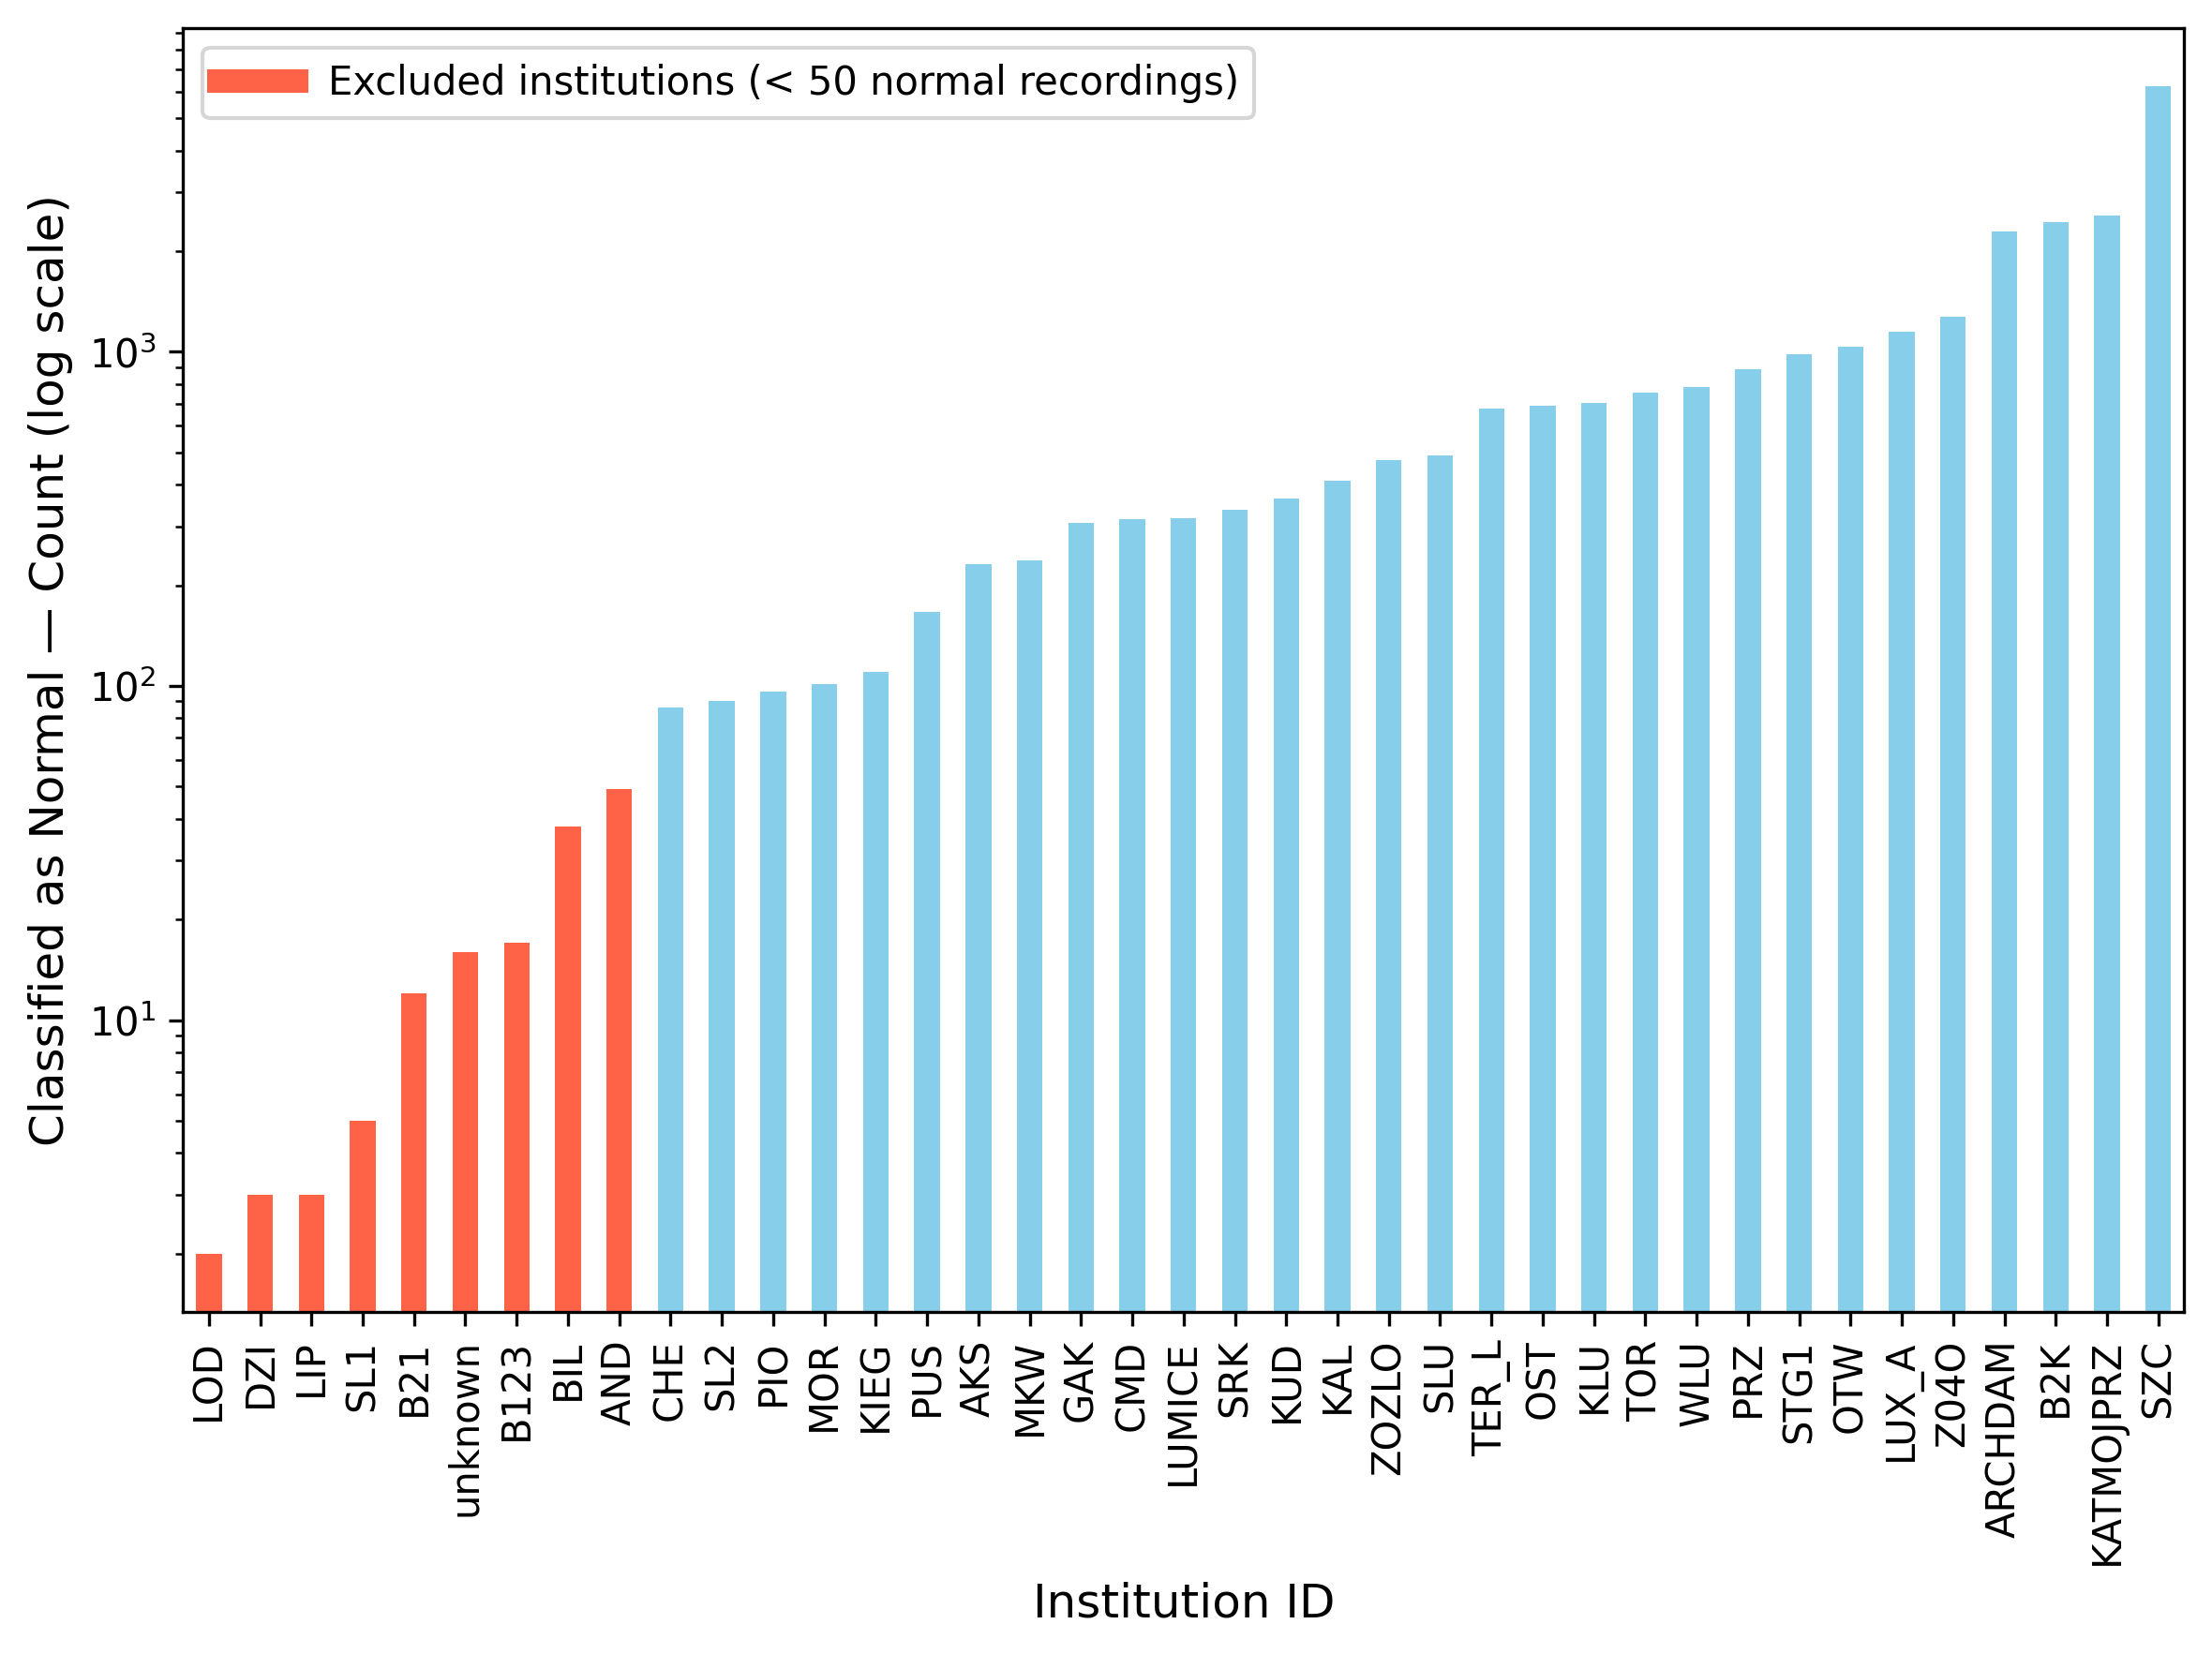
\includegraphics[width=\textwidth]{results/ELM19_excluded_institutions_normal_recordings.png}
            \caption{Number of recordings classified as normal per institution.}
            \label{fig:normal_hist_excluded}
          \end{subfigure}
          \hfill
          \begin{subfigure}[t]{0.48\textwidth}
            \centering
            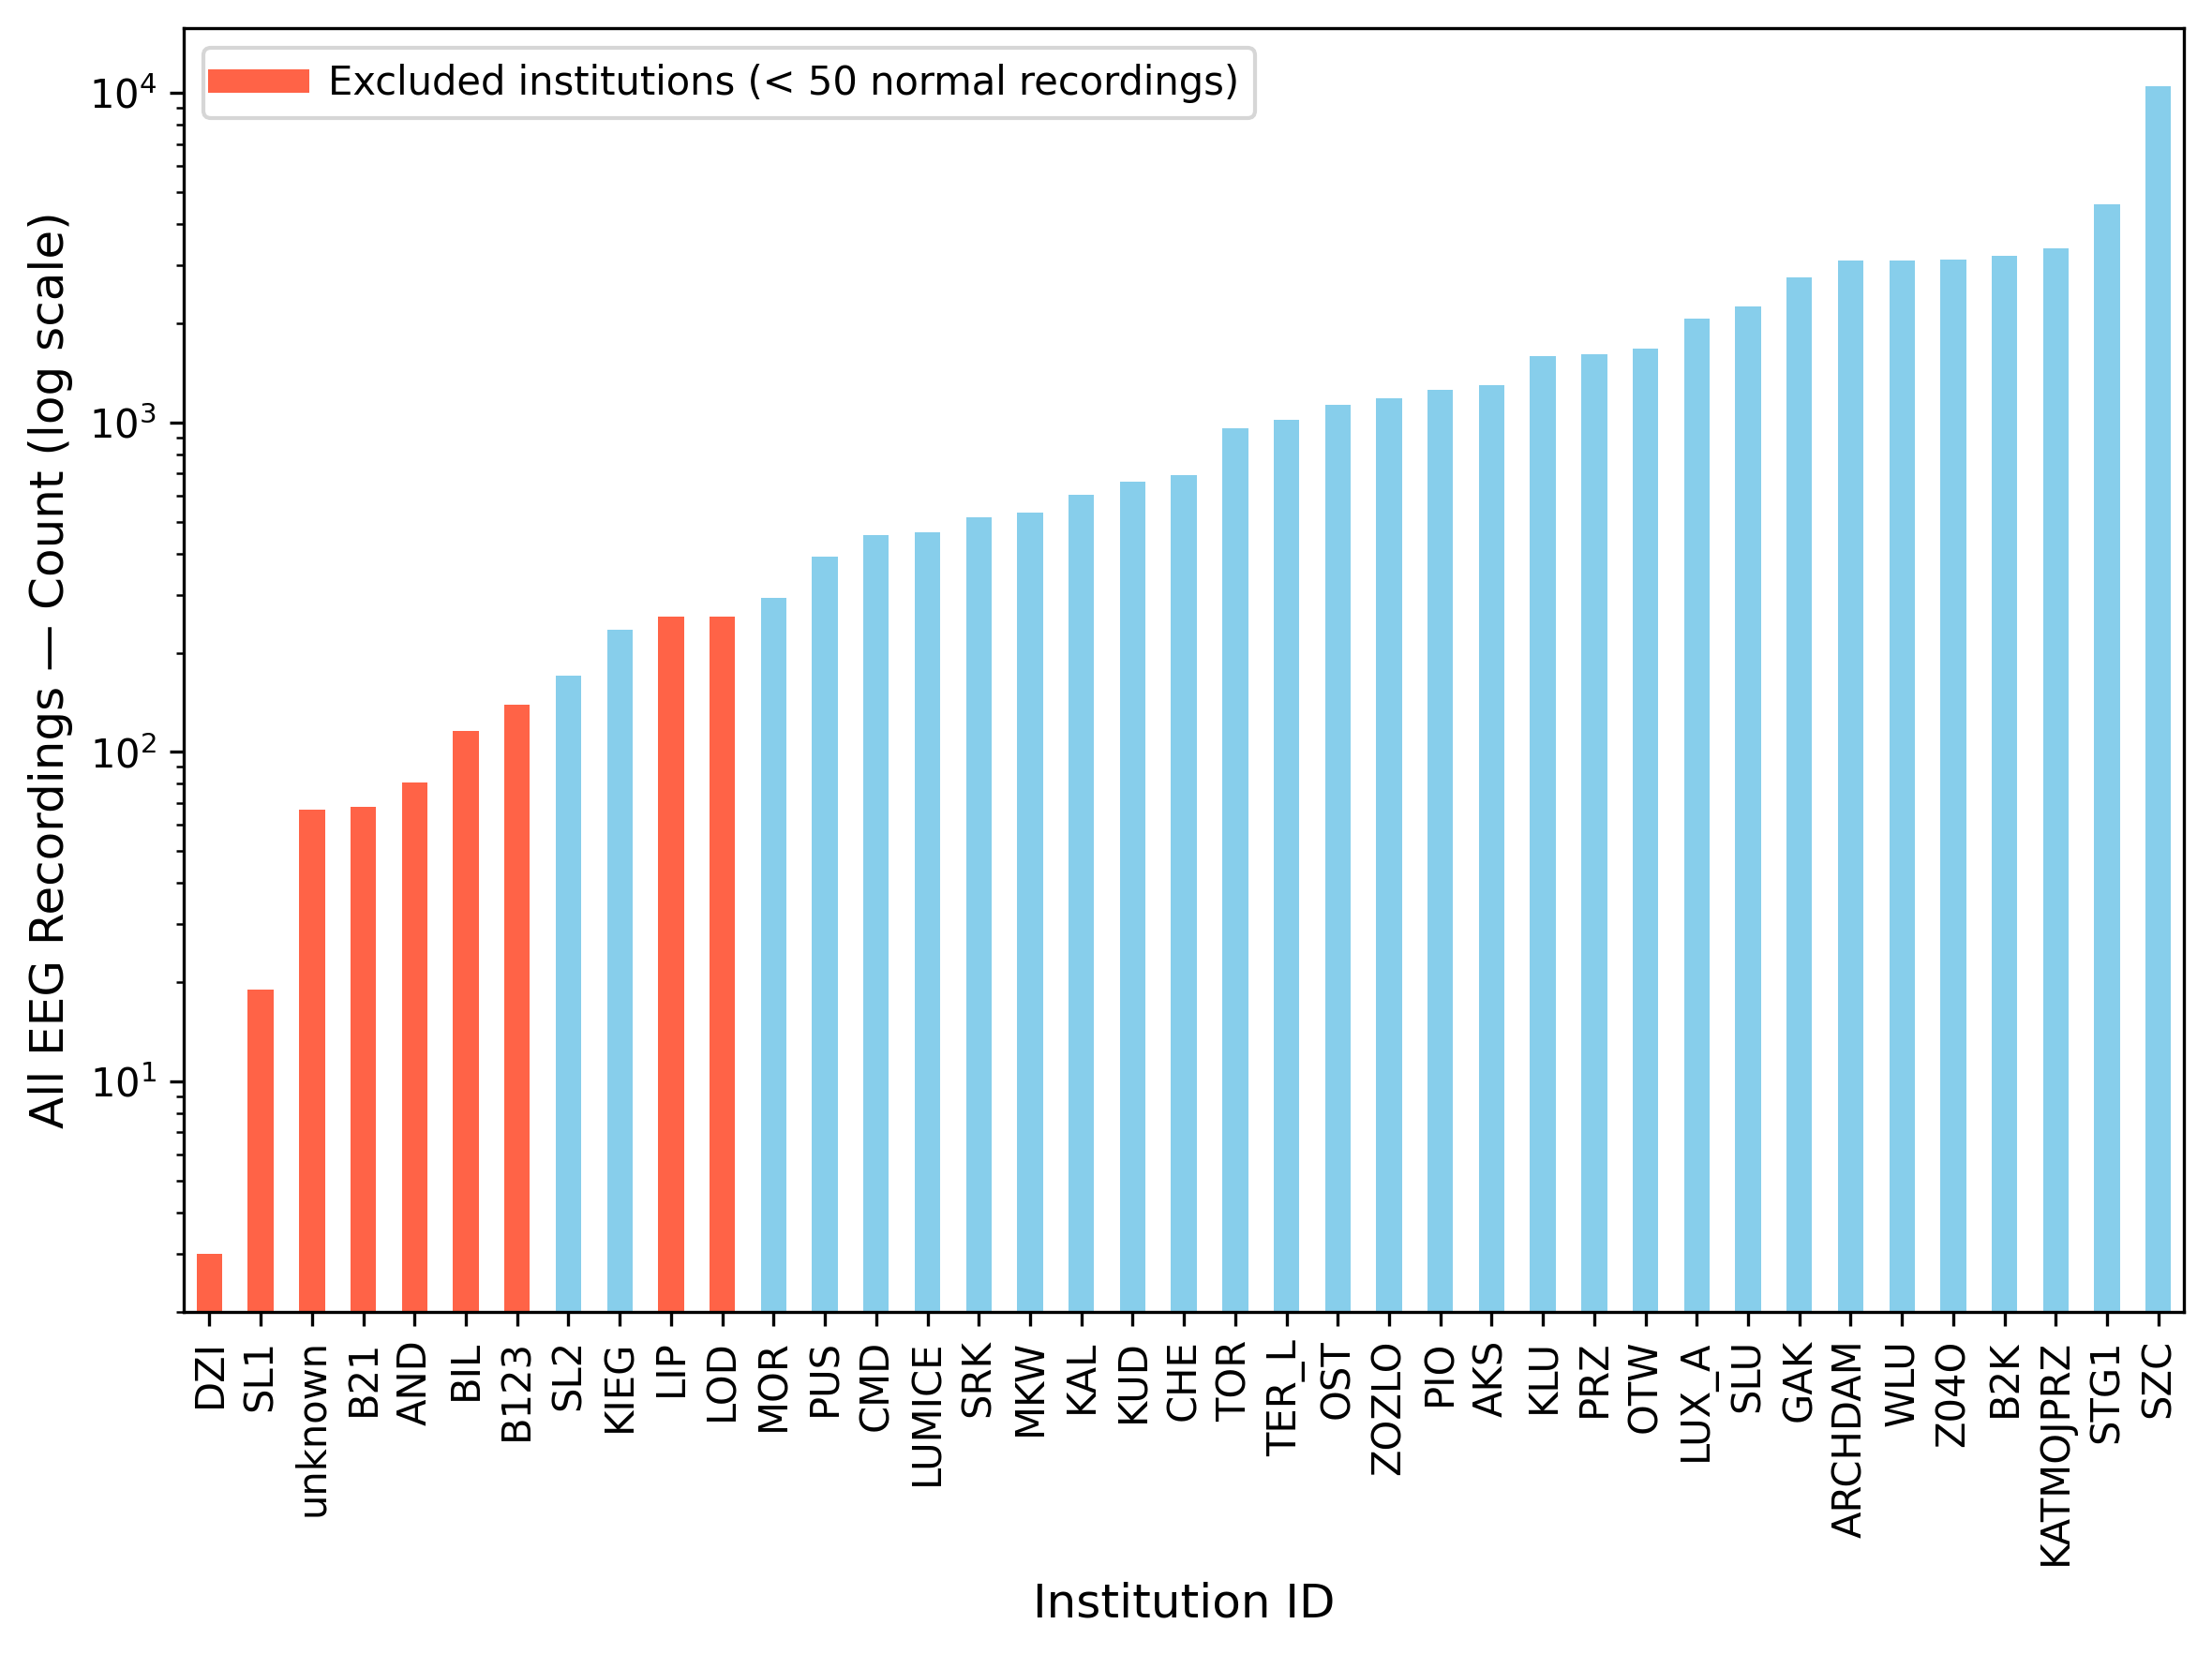
\includegraphics[width=\textwidth]{results/ELM19_excluded_institutions_all_recordings.png}
            \caption{Total number of recordings (normal and pathological) per institution.}
            \label{fig:total_hist_excluded}
          \end{subfigure}
          \caption{Distribution of recordings across medical institutions.}
          \label{fig:institution_histograms}
        \end{figure}

        \subsubsection{Characteristics of the Final ELM19 sample}
        After filtering, the final ELM19 dataset contains 54,779  EEG recordings from the remaining 30 medical institutions. The patients' ages range from 16 to 70. There are 28,960 females (52.9\%) in the gender distribution. The dataset is well balanced, with 26,568 (48.5\%) recordings classified as normal and 28,211 (51.5\%) classified as pathological.

        \subsection{EEG Acquisition Parameters, Data Format, and Recording Protocols}
        The EEG signals were acquired using the standard 10-20 system with 19 channels allocated as follows: Fp1, Fp2, F7, F3, Fz, F4, F8, T3, C3, Cz, C4, T4, T5, P3, Pz, P4, T6, O1, and O2. The data were recorded with original sampling frequencies ranging from 200 to 500\,Hz and stored in the European Data Format (EDF) \cite{Kemp1992}. The recordings originate from routine clinical diagnostic sessions. Consequently, the exact procedures could vary between institutions and patients, though they often included standard tasks such as photostimulation, hyperventilation, and periods of eye-opening and closing.          

    \section{EEG Data Preprocessing}
        To prepare the ELM19 data for further feature extraction, a standardized preprocessing pipeline was applied. The aim of this step was to remove noise and artifacts that were present in the data. All preprocessing steps were implemented using custom scripts in Python, using the MNE-Python library \cite{Gramfort2013}.

        The EEG signals were first filtered using Butterworth filters to eliminate frequencies commonly affected by muscle artifacts and slow drift. Specifically, a high-pass filter with a cutoff at 0.1\,Hz and less than 1\,dB passband ripple above 0.5\,Hz was applied, along with a low-pass filter with a cutoff at 40\,Hz,  which decreased frequencies by at least 20\,dB above 50\,Hz while keeping a passband ripple below 1\,dB. Next, to eliminate power-line noise, a notch filter with a frequency of 50\,Hz and a quality factor $Q = 5$ was used. Afterward, all signals were re-referenced to a common average reference, which helps to reduce the impact of any noisy electrode, and resampled to 100\,Hz to ensure a uniform sampling rate across all facilities. Frames of adjacent 6-second segments were extracted from the preprocessed signals. Frames with voltages higher than 800\,$\mu$V or flat-line channels were rejected as artifacts.
        
    \section{Feature Extraction}
    \label{sec:features}
        For the extraction of features, this study utilized the methodology described in prior work~\cite{Poziomska2024}. Several types of features were extracted from each 6-second EEG segment and later aggregated using the median across all frames in each recording.

        For frequency-domain features, 14 overlapping frequency bands ($f_b$) were defined: \(\left[0.5, 2\right]\), \(\left[1, 3\right]\), \(\left[2, 4\right]\), \(\left[3, 6\right]\), \(\left[4, 8\right]\), \(\left[6, 10\right]\), \(\left[8, 13\right]\), \(\left[10, 15\right]\), \(\left[13, 18\right]\), \(\left[15, 21\right]\), \(\left[18, 24\right]\), \(\left[21, 27\right]\), \(\left[24, 30\right]\), and \(\left[27, 40\right]\)\,Hz. These bands cover the standard EEG frequency ranges: delta~(\(\delta\)), theta~(\(\theta\)), alpha~(\(\alpha\)), and low and high beta~(\(\beta\)).
        
        Three groups of features were extracted: time-domain covariance matrices, frequency-domain coherence features, and frequency-band power features. While the coherence and power features depended on the selected frequency bands, the covariance features were calculated directly in the time domain.


        \subsection{Time-domain covariance matrices}
            Standard Euclidean operations are insufficient for time-domain covariance matrices between EEG channels, which lie on a Riemannian manifold \cite{congedo2013Riemannian, tibermacine2024riemannian}. The covariance matrices were constructed using the Riemannian metric to produce a representative matrix that captures the spatial relationships between EEG channels \cite{Moakher2005}. Then, this matrix is projected onto the tangent space of the manifold to create a feature vector composed of the different components from the symmetric covariance matrix (either the upper or lower triangle) \cite{Lotte2018}. This procedure creates 190 features per recording that efficiently capture the spatial covariance structure of the EEG signal. The pyRiemann\footnote{\url{https://pyriemann.readthedocs.io/}} library was used to compute these features from beginning to end.

        \subsection{Frequency-domain power features}
            The power spectral densities~(PSD) corresponding to the selected frequency bands, represented as \(S_{xx}(f_b)\), where \(x\) is the channel index, are the most fundamental frequency-domain features. The multitaper method~\cite{Thomson1982}, which yields a reliable spectral estimate, is used to estimate these PSDs. After estimation, the PSDs are normalized such that their sum across all channels and frequency bands equals one within each frame. This procedure results in 266 power features per recording extracted from the EEG signals using the MNE-Python library~\cite{Gramfort2013}.

        \subsection{Frequency-domain Coherence Features}
            Band-wise coherence features are derived from the cross-spectral densities, \(S_{xy}(f_b)\). These cross-spectra are used to estimate coherence between EEG channels within each frequency band according to the formula (Eq.~\ref{eq:coherence}): 
            
            \begin{equation}
            \label{eq:coherence}
            C_{xy}(f_b) = \frac{|S_{xy}(f_b)|}{\sqrt{S_{xx}(f_b) \cdot S_{yy}(f_b)}}
            \end{equation}

            \noindent
            where \(S_{xx}(fb)\) and \(S_{yy}(fb)\) are the power spectral densities of channels \(x\) and \(y\), respectively. Since the coherence matrix is symmetric with ones on the diagonal, only the sub-diagonal elements are retained, resulting in 2,394 coherence features per recording.

        \subsection{Final feature set}
            A total of 2,850 features are included in the final feature set, which was designed to capture multiple aspects of the EEG signal, including its spatial structure in the time domain, its spectral power characteristics across a wide frequency range, and the  connectivity between all electrode pairs.

    \section{Investigating the Site Effect using Machine Learning}
    \label{sec:machine_learning}
            The site effect can arise from complex feature interactions, making them hard to detect with simple observation. Machine learning models used in neuroscreening are capable of learning underlying structures in high-dimensional data, which can lead them to fit to site-specific patterns. Thus, in order to quantify the site effect, a supervised machine learning framework was employed with a specific task—to classify the source hospital of an EEG recording based on its features. For this multi-class classification, the institution ID served as a target variable, and the 2,850 covariance, coherence, and power features (described in \autoref{sec:features}) were used as the model's input. 
        \subsection{Classifier Selection and Hyperparameter Tuning}
            For this task, the CatBoost classifier \cite{Prokhorenkova2017} was selected. Its strengths include the ability to effectively handle high-dimensional data, its efficiency in multi-class classification, and robustness against overfitting. Another valuable aspect, common to tree-based models, is its relatively good interpretability, which is important for understanding the factors driving site classification.  Its hyperparameters were specifically adjusted for this task using the Optuna framework\footnote{Available at \url{https://optuna.org/}} \cite{Akiba2019}.

        \subsection{Performance Evaluation}
            To assess model performance, the 5-fold stratified cross-validation was applied. Given the significant class imbalance, stratification by hospital ID ensured that the proportion of recordings from each institution remained constant across all folds. The Matthews Correlation Coefficient (MCC) was used as the evaluation metric. The one-vs-rest approach was used to compute the individual MCC scores for each hospital class. Specifically, the MCC for a given hospital was calculated by treating that hospital as the positive class and all other hospitals as the negative class (Eq.~\ref{eq:binary_mcc}).
    
            \begin{equation}
            \label{eq:binary_mcc}
            MCC = \frac{tp \times tn - fp \times fn}{\sqrt{(tp + fp)(tp + fn)(tn + fp)(tn + fn)}}
            \end{equation}
            
            \noindent
            where \( tp \), \( tn \), \( fp \), and \( fn \) are respectively the number of true positives, true negatives, false positives, and false negatives. 
            
            Additionally, an overall MCC value was reported, calculated using the multiclass generalization of MCC. For a \(K\)-class problem, let \(\mathbf{C} \in \mathbb{N}^{K \times K}\) be the confusion matrix, where \(C_{ij}\) denotes the number of samples known to be in class \(i\) (true class) and predicted to be in class \(j\) (predicted class). To define the multiclass MCC, the following intermediate variables are used:
            \begin{itemize}
                \item \( t_k = \sum_{j=1}^{K} C_{kj} \) --- the total number of times class \(k\) truly occurred (i.e., the sum of row \(k\) of \(\mathbf{C}\)).
               \item \( p_k = \sum_{i=1}^{K} C_{ik} \) --- the total number of times class \(k\) was predicted (i.e., the sum of column \(k\) of \(\mathbf{C}\)).
               \item \( c = \sum_{k=1}^{K} C_{kk} \) --- the total number of samples correctly predicted (i.e., the sum of the main diagonal of \(\mathbf{C}\)).
               \item \( s = \sum_{i=1}^{K} \sum_{j=1}^{K} C_{ij} \) --- the total number of samples.
            \end{itemize}
            
            \noindent
            The multiclass MCC is then given by (Eq.~\ref{eq:multiclass_mcc}):
            
            \begin{equation}
            \label{eq:multiclass_mcc}
            \text{MCC} = \frac{
               c s - \sum_{k=1}^{K} p_k t_k
            }{\sqrt{
               \left(s^2 - \sum_{k=1}^{K} p_k^2\right)
               \left(s^2 - \sum_{k=1}^{K} t_k^2\right)
            }}
            \end{equation}

        \subsection{Feature importance Analysis}
            
            

    \section{Data Harmonization}
        \subsection{Selection of Harmonization Technique}
        \subsection{Application of Harmonization}
        \subsection{Evaluating Harmonization Effectiveness}

    \section{Neuroscreening Task}
        \subsection{Task Definition}
        \subsection{Labeling}
        \subsection{Predictive Model}
        \subsection{Performance Evaluation}
        \subsection{Comparison (Original vs. Harmonized Data)}
        

\chapter{Results}
    \section{EEG Data Overview (ELM19)}
        % Summary statistics of final dataset
    \section{Site Effect Demonstration}
        The CatBoost classifier, configured and validated as described in Chapter~\ref{chap:methods} (Section~\ref{sec:machine_learning}) demonstrated a strong ability to classify the hospital of origin from extracted EEG features. The model achieved an overall MCC value of \({0.865 \pm 0.003}\) across the 30 ELM19 institutions in the 5-fold stratified cross-validation. The averaged normalized confusion matrices are presented in the appendix (see Figure~\ref{fig:confusion_matrix_appendix}), while the averaged one-vs-rest MCC scores for each hospital are illustrated in Figure~\ref{fig:hospital_classification_mcc_all_features}. While the figure displays only the mean MCCs for visual clarity, the complete mean values along with their standard deviations across the 5 cross-validation folds are provided in the appendix (see Table~\ref{tab:mean_mcc_per_hospital}).

        \begin{figure}[htbp]
        \centering
        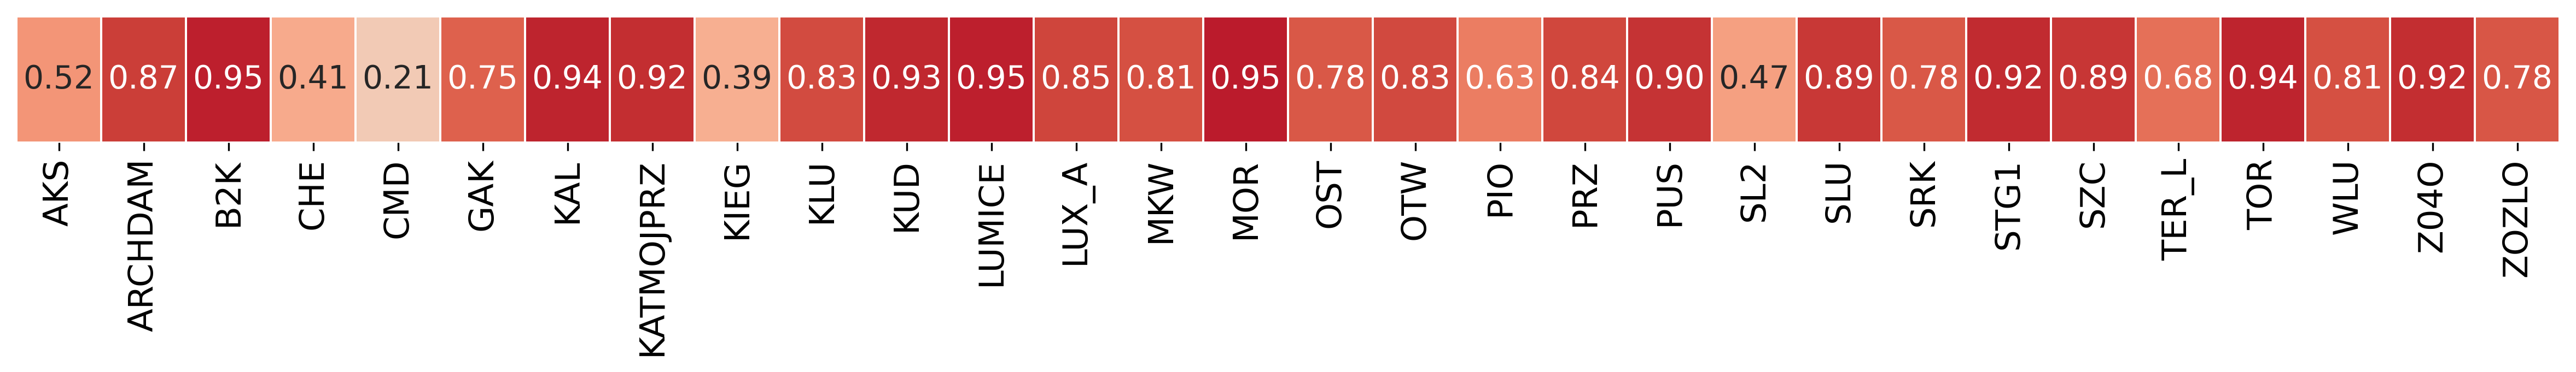
\includegraphics[width=\textwidth]{results/hospital_classification_avg_mcc_per_class.png}
        \caption{Average MCC for Each Class (5-Fold CV)}
        \label{fig:hospital_classification_mcc_all_features}
        \end{figure}

        The model performed very well for the majority of hospitals, with 23 out of 30 achieving average MCC scores above 0.7. However, a small subset of institutions—AKS, CHE, KIEG, and SL2—performed poorly, with average MCC scores ranging from 0.39 to 0.52, making them significantly more difficult to classify. Furthermore, with the lowest average MCC score of 0.21, one institution, CMD, stood out for its extremely poor classification performance.

    \section{Key Features Differentiating Sites}
        
    \section{Impact of Individual Feature Groups on Site Classification}        
        The next step of the analysis was to understand the contributions of different feature types. The features were divided into three categories: time-domain covariance, power spectral densities, and band-wise coherences. 

        Firstly, three separate models were trained, each using only features from one of the three groups (covariance, power, or coherence), to check the performance that could be achieved with each group individually. The average MCC scores across the five folds for these models are shown in Figure~\ref{fig:hospital_classification_mcc_selected_features}. 

        \begin{figure}[htbp]
        \centering
        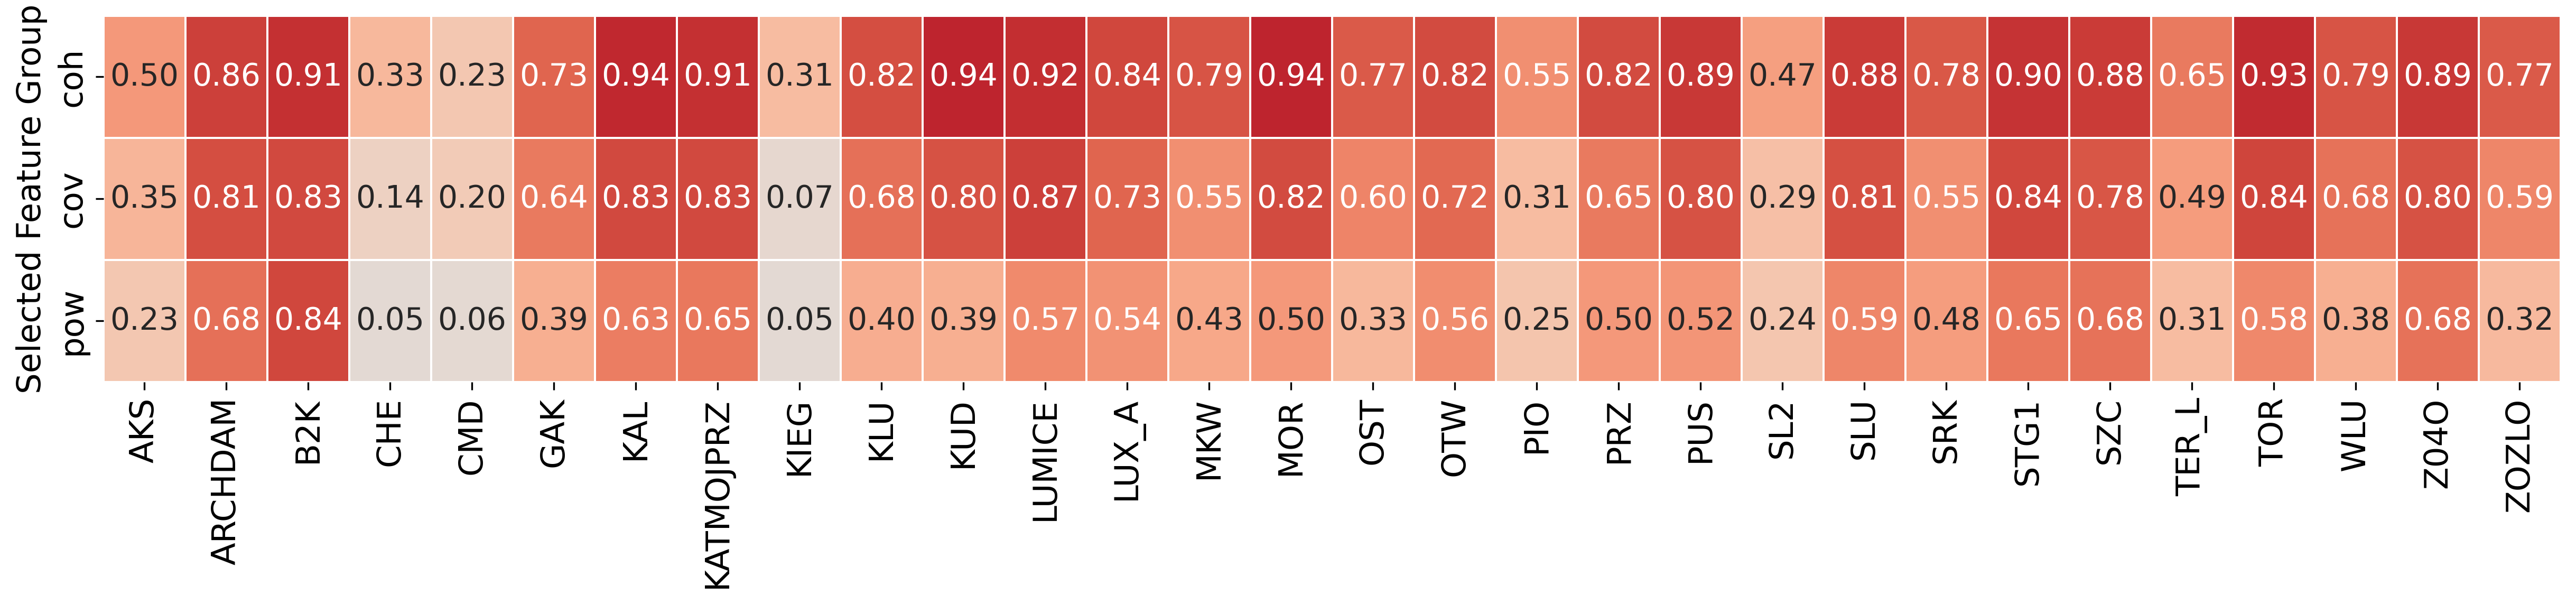
\includegraphics[width=\textwidth]{results/selected_features_group_hospital_classification_avg_mcc_per_class.png}
        \caption{Average MCC per Hospital (5-Fold CV): Performance with Individual Feature Group}
        \label{fig:hospital_classification_mcc_selected_features}
        \end{figure}
        
        Next, three further models were trained, each excluding features from one of the three groups, to see how the model functions without that particular group of features. The average MCC scores across the five folds for these models are shown in Figure~\ref{fig:hospital_classification_mcc_exluded_features}

        \begin{figure}[htbp]
        \centering
        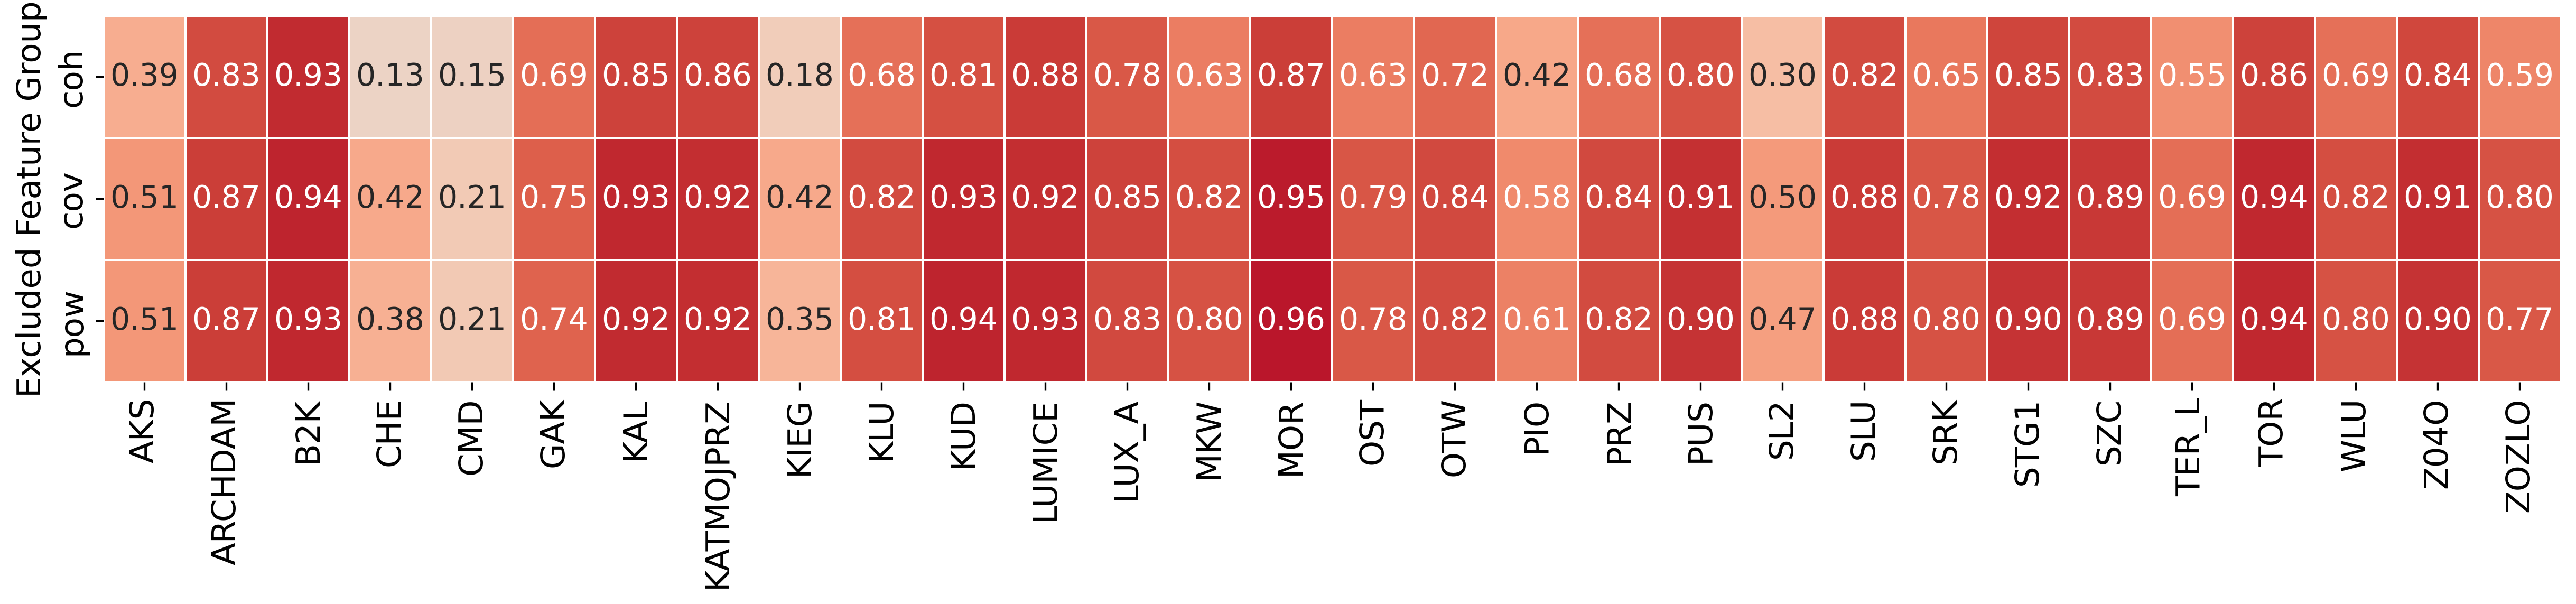
\includegraphics[width=\textwidth]{results/excluded_features_group_hospital_classification_avg_mcc_per_class.png}
        \caption{Average MCC per Hospital (5-Fold CV): Performance with Feature Group Exclusion}
        \label{fig:hospital_classification_mcc_exluded_features}
        \end{figure}

        The results from both Figure~\ref{fig:hospital_classification_mcc_selected_features} and Figure~\ref{fig:hospital_classification_mcc_exluded_features} show that a model trained only on covariance or coherence features achieved performance comparable to a model trained on all available features. In contrast, the model that was trained only on the power features performed significantly worse.



    \section{Harmonization Impact on Classification Performance}
        % Site classification performance on harmonized data, direct comparison (before vs. after), visualizations of feature distributions.

    \section{Impact on Clinical Prediction Model}
        % - Results for original data
        % - Results after feature modification (or overall harmonization)

\chapter{Discussion}
    \section{Summary of Results}
        % - Key findings regarding EEG features
        % - Effectiveness of the GBE model in distinguishing hospitals

    \section{Study Limitations and Possible Improvements}
        % - Potential errors and constraints
        % - Future research directions

\chapter{Summary} 
        % - Summary of the study and answers to research questions
        % - Practical implications of the results


% --- Bibliography ---
\bibliographystyle{IEEEtran} 
\bibliography{bibliography}

\appendix
\chapter{Additional Figures and Tables}
\label{app:additional_figures}
\begin{figure}[htbp]
    \centering
    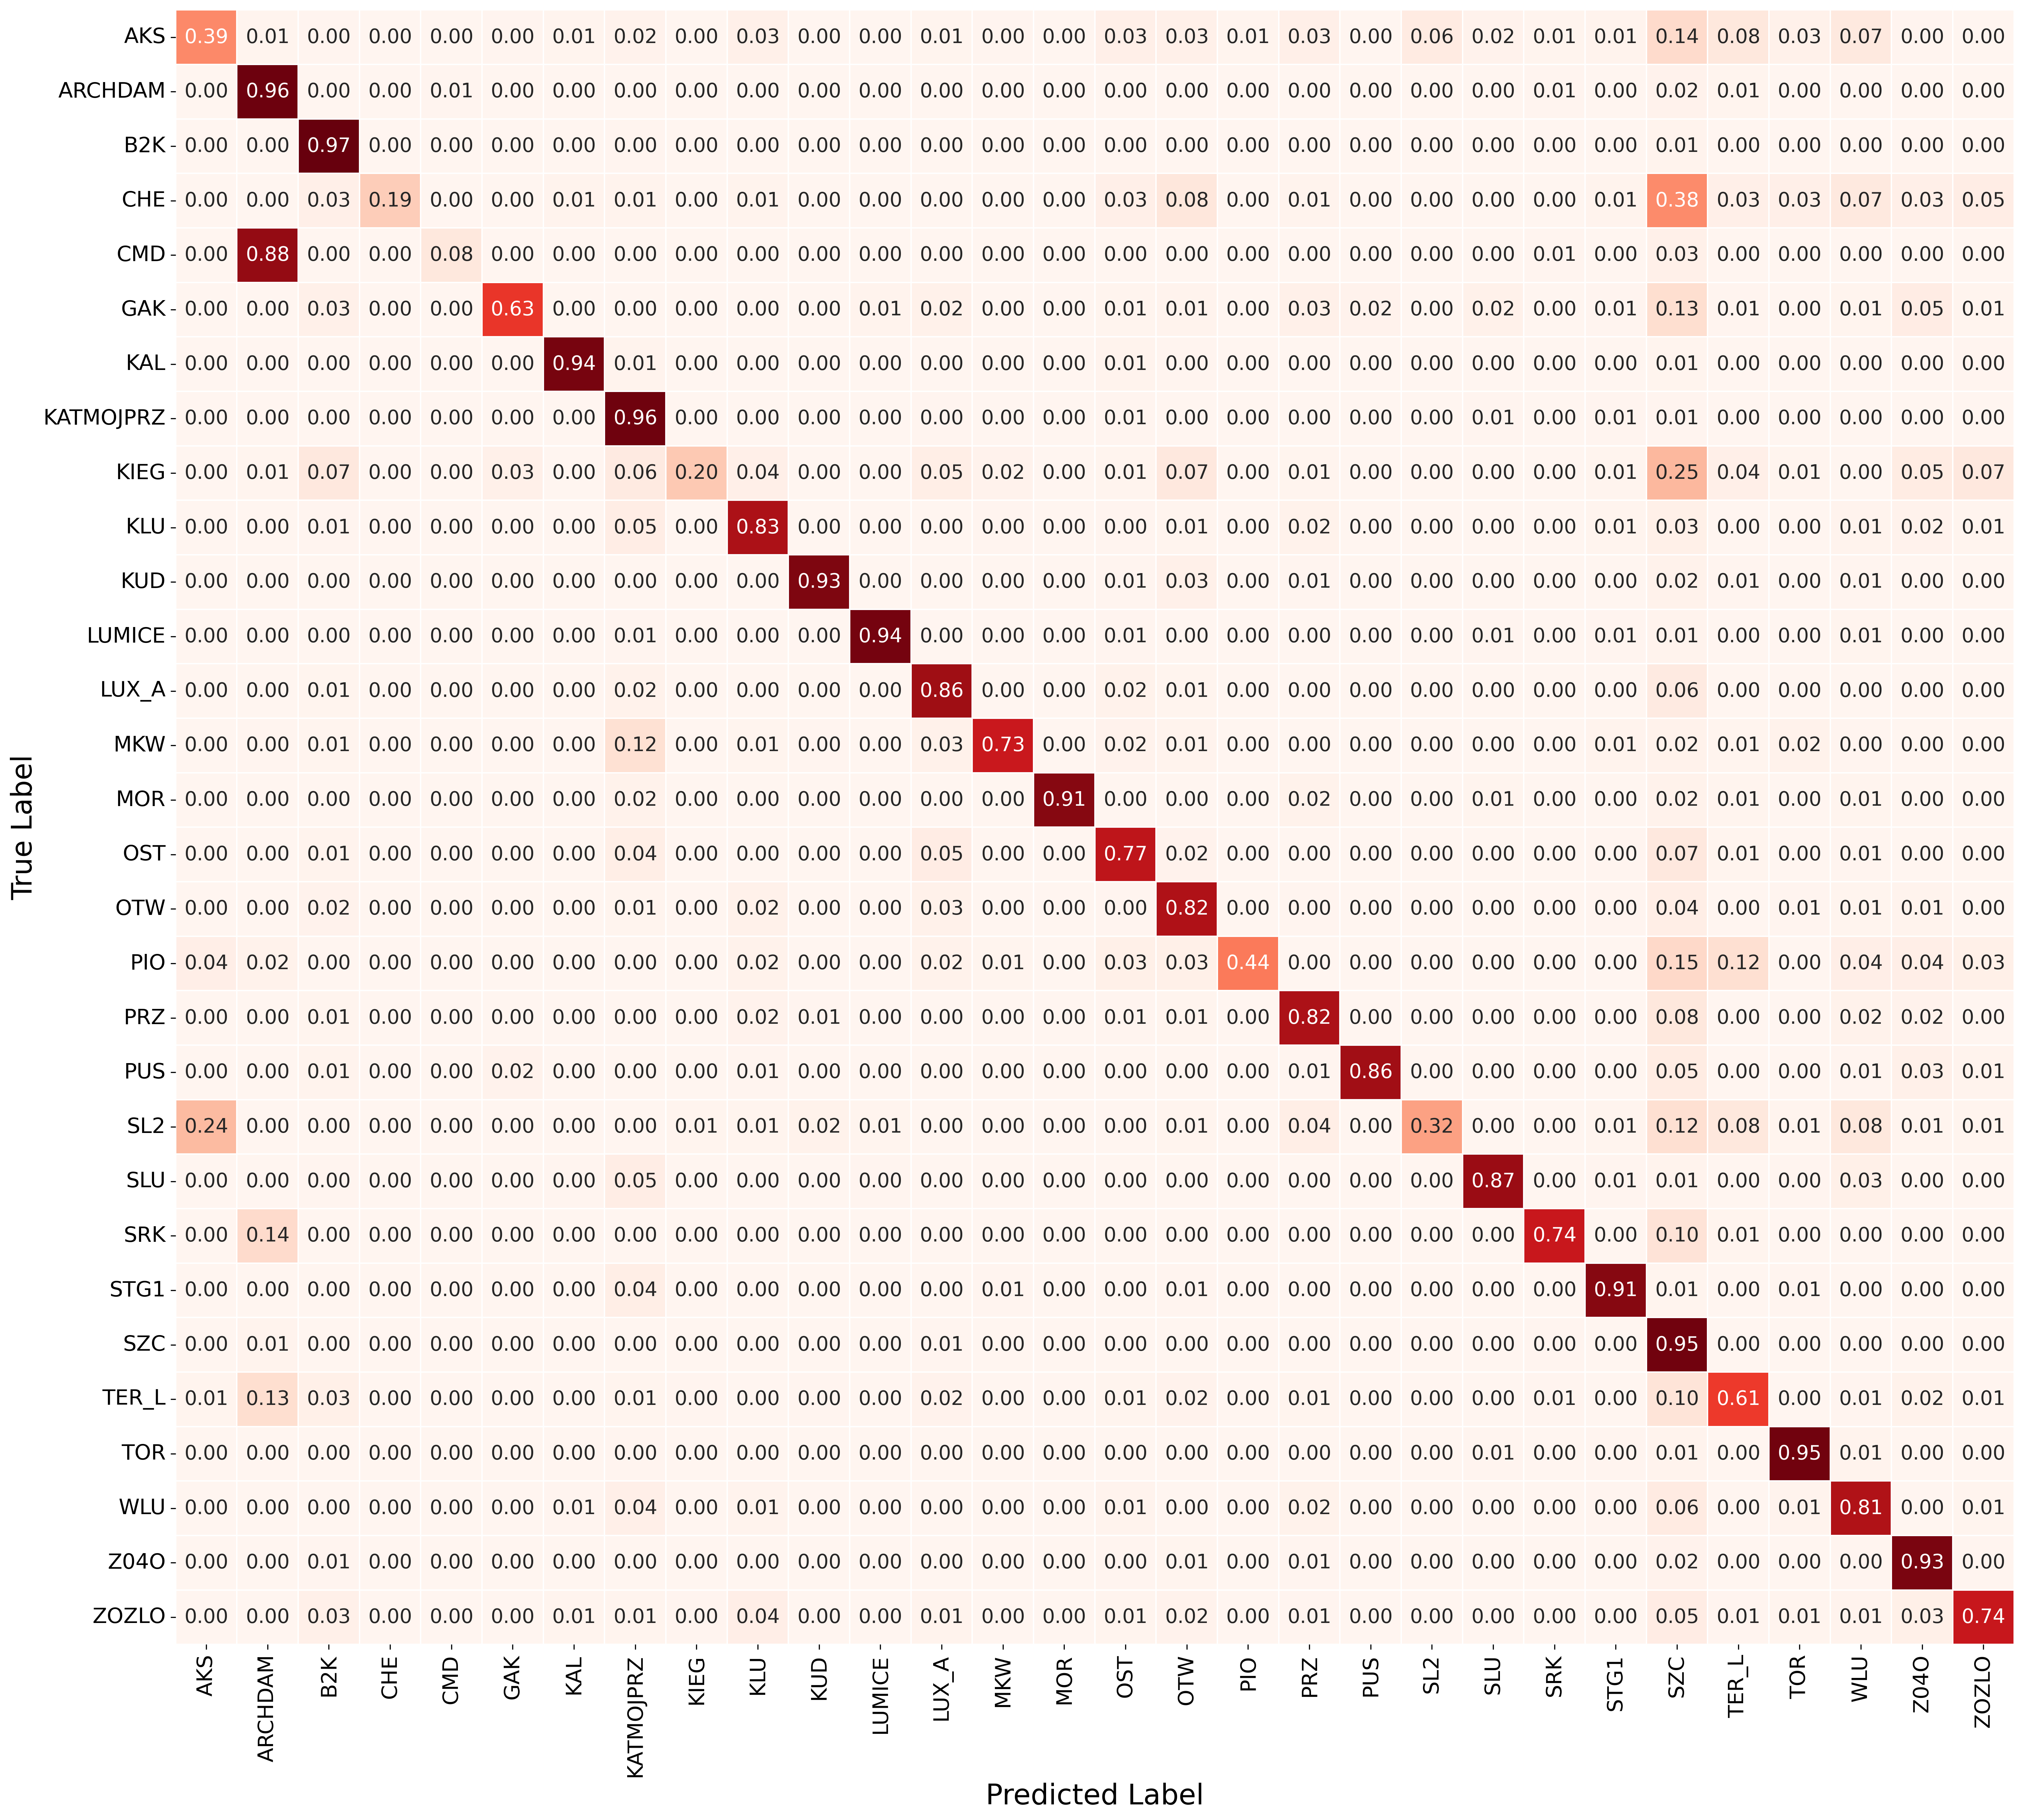
\includegraphics[width=\linewidth]{results/hospital_classification_avg_confusion_matrix.png}
    \caption{Averaged normalized confusion matrix across the 30 ELM19 institutions in the 5-fold stratified cross-validation.}
    \label{fig:confusion_matrix_appendix}
\end{figure}

\begin{table}[ht]
    \centering
    \caption{Mean MCC values and standard deviations for each hospital (5-fold cross-validation).}
    \label{tab:mean_mcc_per_hospital}
    \begin{tabular}{|l|c|c|}
    \hline
    \textbf{Hospital} & \textbf{Mean MCC} & \textbf{Std. Dev.} \\
    \hline
    AKS          & 0.517 & 0.117 \\
    ARCHDAM      & 0.872 & 0.014 \\
    B2K          & 0.952 & 0.006 \\
    CHE          & 0.407 & 0.113 \\
    CMD          & 0.207 & 0.047 \\
    GAK          & 0.748 & 0.014 \\
    KAL          & 0.941 & 0.030 \\
    KATMOJPRZ    & 0.918 & 0.012 \\
    KIEG         & 0.390 & 0.079 \\
    KLU          & 0.828 & 0.015 \\
    KUD          & 0.933 & 0.017 \\
    LUMICE       & 0.947 & 0.034 \\
    LUX\_A       & 0.851 & 0.016 \\
    MKW          & 0.809 & 0.034 \\
    MOR          & 0.954 & 0.035 \\
    OST          & 0.781 & 0.016 \\
    OTW          & 0.830 & 0.010 \\
    PIO          & 0.626 & 0.098 \\
    PRZ          & 0.844 & 0.016 \\
    PUS          & 0.899 & 0.048 \\
    SL2          & 0.467 & 0.112 \\
    SLU          & 0.890 & 0.026 \\
    SRK          & 0.780 & 0.036 \\
    STG1         & 0.922 & 0.010 \\
    SZC          & 0.893 & 0.005 \\
    TER\_L       & 0.682 & 0.025 \\
    TOR          & 0.938 & 0.015 \\
    WLU          & 0.805 & 0.015 \\
    Z04O         & 0.915 & 0.012 \\
    ZOZLO        & 0.782 & 0.048 \\
    \hline
    \end{tabular}
\end{table}

% =========================================================================
% End of the Document Content
% =========================================================================
\end{document}
